\question{Câu 3}

Cho mạch điện như ở Hình 3 sau:

\begin{figure}[H]
	\centering
	
\includegraphics[width=.6\linewidth]{./my-chapters/my-images/Question3/debai.png}
	\caption*{Hình 3.}
\end{figure}

\answer{a}{Giả sử OPAMP là lí tưởng. Tím liên hệ giữa $V_{o}$ với $V_{1}$ và $V_{2}$.}

\begin{itemize}[label=-]
	\item Xét tầng 1:
	\[ V_{o1} = -\dfrac{2R}{R} V_{1} = -2V_{1} \]
	
	\item Xét tầng 2:
	\[ V_{o} = -\dfrac{4R}{R}V_{o1} - \dfrac{4R}{2R}V_{2} \]
	
	\item Xét toàn mạch:
	
	\begin{center}
		\finalresult{V_{o} = 8V_{1} - 2V_{2}}
	\end{center}
	
	\item Mô phỏng mạch:
	
	\begin{figure}[H]
		\centering
		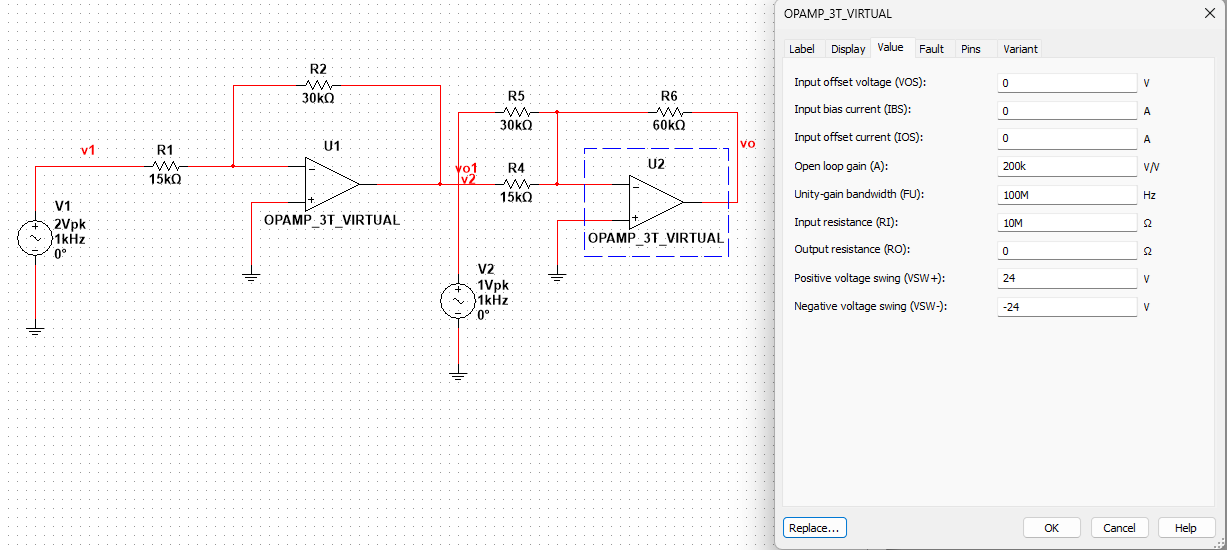
\includegraphics[width=.9\linewidth]{./my-chapters/my-images/Question3/a_machmophong_ideal.png}
		\caption{Mô phỏng liên hệ giữa $V_{o}$ với $V_{1}$ và $V_{2}$ với OPAMP lý tưởng.}
	\end{figure}
	
	\begin{figure}[H]
		\centering
		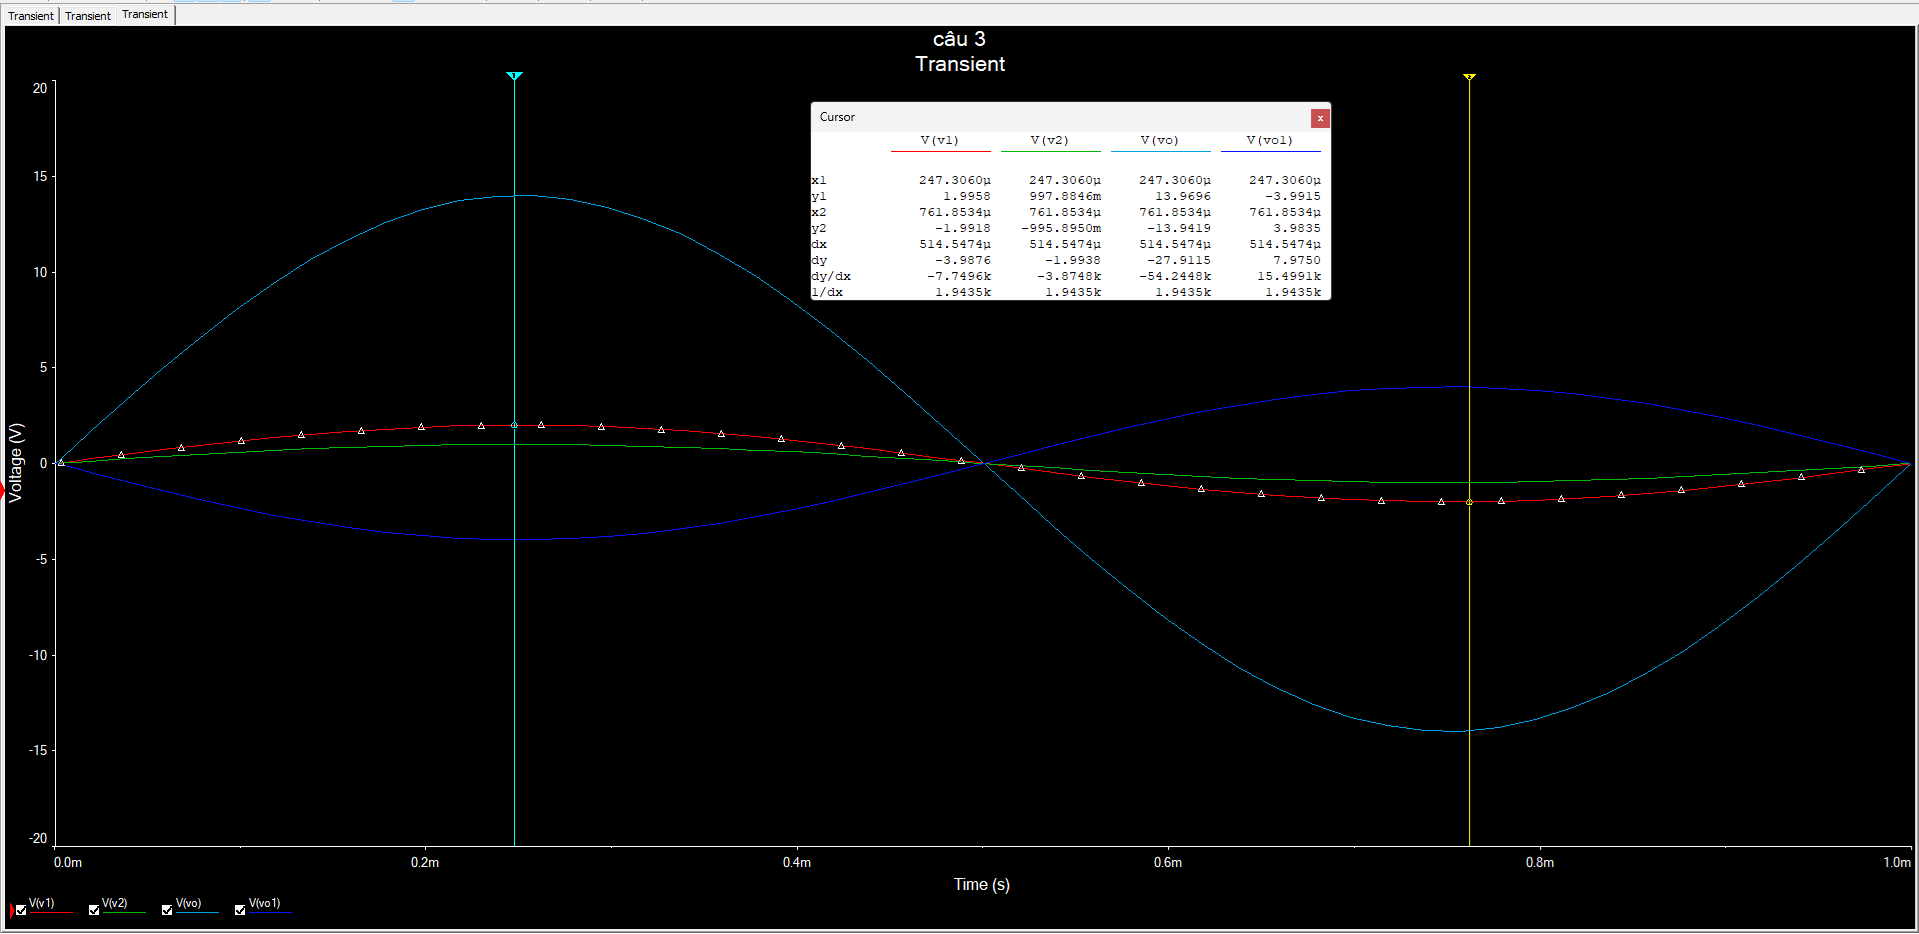
\includegraphics[width=.9\linewidth]{./my-chapters/my-images/Question3/a_songmophong_ideal.png}
		\caption{Kế quả của mạch liên hệ giữa $V_{o}$ với $V_{1}$ và $V_{2}$ với OPAMP lý tưởng.}
	\end{figure}
	
	\begin{minipage}{.7\linewidth}
		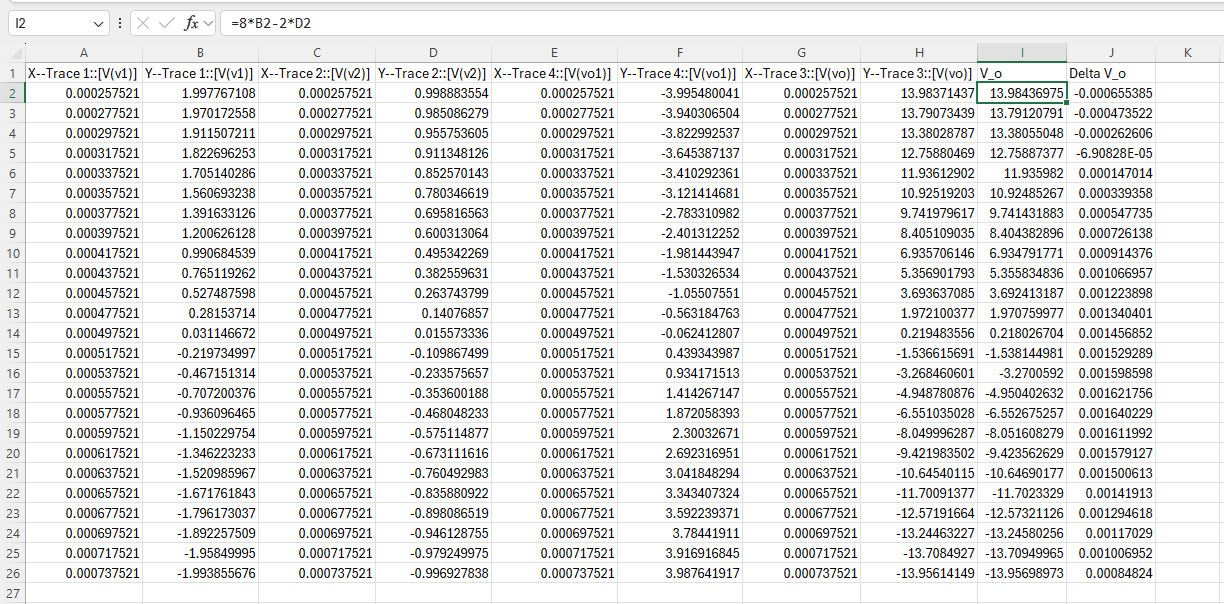
\includegraphics[width=\linewidth]{./my-chapters/my-images/Question3/a_thongso.png}
	\end{minipage}
	\begin{minipage}{.3\linewidth}
		\begin{itemize}[label=-]
			\item \finalresult{\Delta V_{o_{max}} = 0.001640229 \,\textsf{V}}
			\item \finalresult{\Delta V_{o_{min}} = -0.000655385 \,\textsf{V}}
		\end{itemize}
	\end{minipage}
	
\end{itemize}

\answer{b}{Giả sử cả 2 OPAMP có $V_{io} = 30\,\mu\textsf{V}$, $I_{io} = 0$, $I_{ib} = 20\,\textsf{nA}$. Tỉm ảnh hưởng của $V_{io}$ lên ngõ ra $V_{o}$. Tìm giá tị của $R$ có thể bỏ qua ảnh hưởng của dòng $I_{ib}$.}

\begin{itemize}[label=-]
	\item Xét tầng 1:
	\begin{itemize}[label=+]
		\item Ảnh hưởng do $V_{os}$ gây ra:
		\[
		{ {\Delta V}}_1=\left(1+\frac{2R}{R}\right)V_{os}=3\times30\,\mu\textsf{V}=90\,\mu\textsf{V}
		\]
		
		\item Ảnh hưởng do $I_{io}$, $I_{ib}$ gây ra:
		\[
		\left\{
		\begin{matrix}
			| I_{+} - I_{-} | = I_{io} 	\\[4pt]
			\dfrac{I_{+} + I_{-}}{2} = I_{ib}
		\end{matrix}
		\right.
		\Rightarrow
		\left\{
		\begin{matrix}
			I_{+} = 20\,\textsf{nA}	\\[4pt]
			I_{-} = 20\,\textsf{nA}
		\end{matrix}
		\right.
		\]
		
		\[ \Rightarrow \Delta V_1 = I_{-} 2R = 40R \,\textsf{nV} \]
		\item Ảnh hưởng lên tầng 1 do $V_{os}$, $I_{ib}$ và $I_{io}$:
		
		\finalresult{V_{o1} = -2 V_{1} \pm 90\,\mu\textsf{V} \pm 40R\,\textsf{nV}}
	
	\end{itemize}
	
	\item Xét tầng 2:
	\begin{itemize}[label=+]
		\item Ảnh hưởng do $V_{io}$ gây ra:
		\[
		 \Delta V_2 = \left( 1 + \frac{4R}{R // 2R} \right) V_{io} = 7 \times 30 \,\mu\textsf{V} = 210\,\mu\textsf{V}
		\]
		
		\item Ảnh hưởng do $I_{io}$, $I_{ib}$ gây ra:
		\[
		\Delta V_2 = I^{-} 4R = 80R\,\textsf{nV}
		\]
		
		\item Ảnh hưởng lên tầng 2 do $V_{os}$, $I_{ib}$ và $I_{io}$:
		
		\finalresult{ V_{o2} = -\dfrac{4R}{R}V_{o1} - \dfrac{4R}{2R}V_{2} \pm 210\,\mu\textsf{V} \pm 80R\,\textsf{nV} }
	\end{itemize}
	
	\item Xét toàn mạch:
	
	\begin{itemize}[label=+]
		\item Ảnh hưởng do tầng 1 gây ra:
		\[
		{ {\Delta V}}_o=-\frac{4R}{R}V_{o1}-\frac{4R}{2R}V_{2}\ \left(-\frac{4R}{2R}V_{2}=0\right)
		\]
		\[
		\Rightarrow{ {\Delta V}}_o=-4{ {\Delta V}}_1=\mp360\,\mu\textsf{V}\mp160R\,\textsf{nV}
		\]
		\item Ảnh hưởng của điều kiện không lý tưởng của Opamp gây ra:
		
		\begin{center}
			$\Rightarrow$ \finalresult{{{\Delta V}}_o=8V_{1}-2V_{2}\pm210\,\mu\textsf{V}\pm80R\,\textsf{nV}\mp360\,\mu\textsf{V}\mp160R\,\textsf{nV}}.
		\end{center}
		
	\end{itemize}
	
	\item Mô phỏng mạch:
	
	\begin{figure}[H]
		\centering
		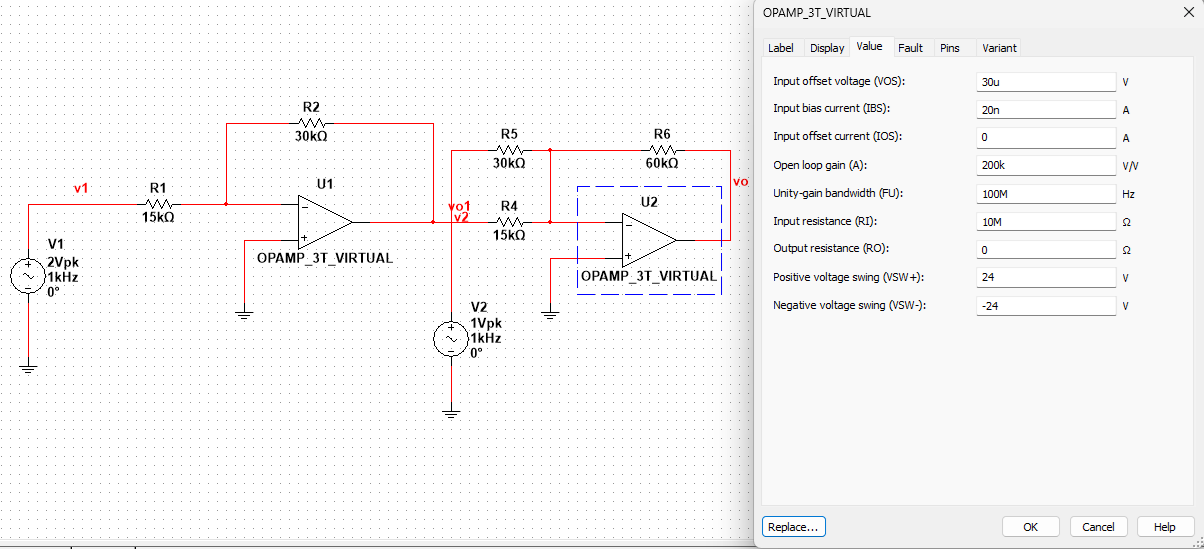
\includegraphics[width=.9\linewidth]{./my-chapters/my-images/Question3/b_mophong1_nonideal.png}
		\caption{Mô phỏng liên hệ giữa $V_{o}$ với $V_{1}$ và $V_{2}$ với OPAMP không lý tưởng.}
	\end{figure}
	
	\begin{figure}[H]
		\centering
		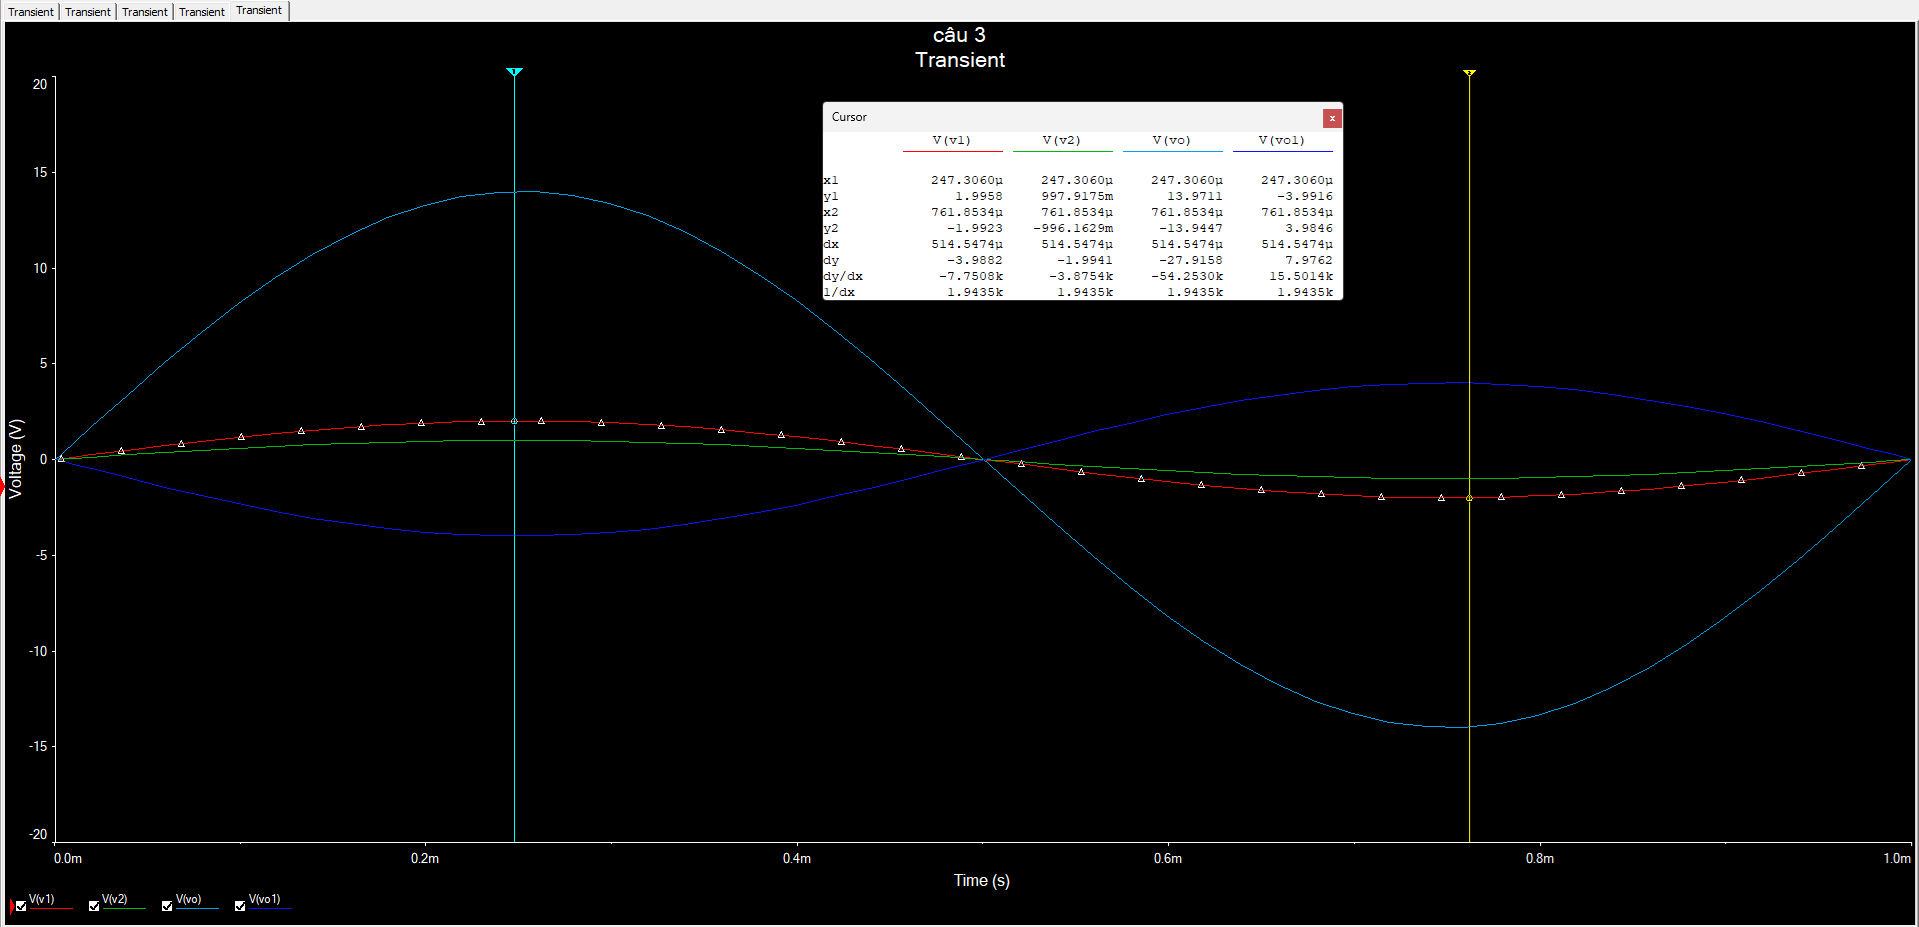
\includegraphics[width=.9\linewidth]{./my-chapters/my-images/Question3/b_songmophong1_nonideal.png}
		\caption{Kết quả mô phỏng liên hệ giữa $V_{o}$ với $V_{1}$ và $V_{2}$ với OPAMP không lý tưởng.}
	\end{figure}
	
	\begin{minipage}{.7\linewidth}
		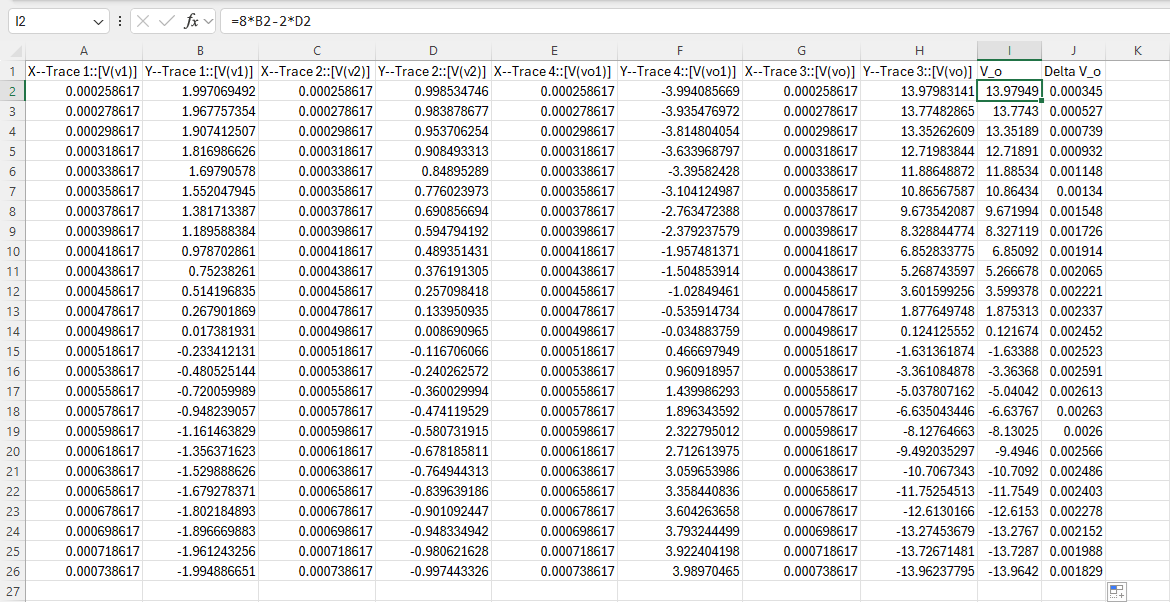
\includegraphics[width=\linewidth]{./my-chapters/my-images/Question3/b_saiso_nonideal_1.png}
	\end{minipage}
	\begin{minipage}{.3\linewidth}
		\begin{itemize}[label=-]
			\item \finalresult{\Delta V_{o_{max}} = 0.002629954 \,\textsf{V}}
			\item \finalresult{\Delta V_{o_{min}} = 0.000344962 \,\textsf{V}}
		\end{itemize}
	\end{minipage}
	
	\item Để loại bỏ ảnh hưởng của $I_{ib}$: Ta có $160R\,\textsf{nV} \ll 210\,\mu\textsf{V}$ để sai số của $I_{ib}$ tác động rất thấp đến sai số ngõ ra mà chỉ có tác động của $V_{os}$ tác động đến sai số là chủ yếu
	\[
	\Rightarrow0.16R\ll21\Rightarrow R\le131.25\,\Omega
	\]
	
	\begin{center}
		$\Rightarrow$ \finalresult{R=130\,\Omega}.
	\end{center}
	
	\begin{figure}[H]
		\centering
		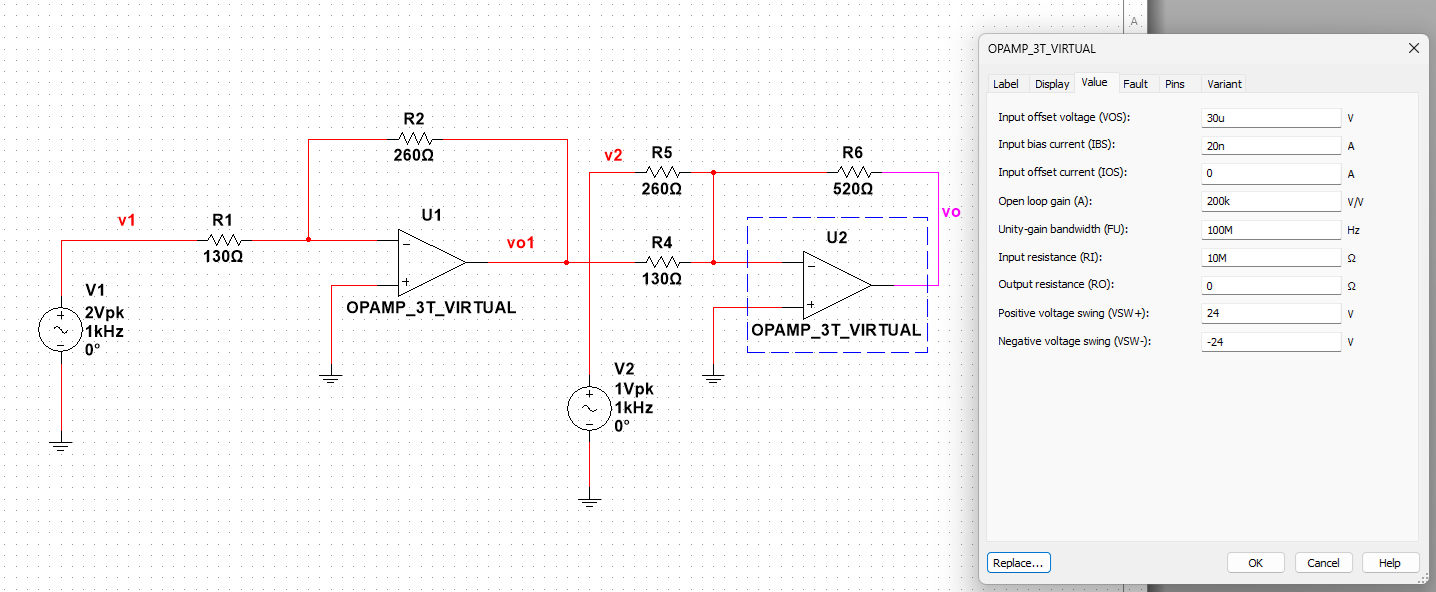
\includegraphics[width=.9\linewidth]{./my-chapters/my-images/Question3/b_mophong2_nonideal.png}
		\caption{Mô phỏng liên hệ giữa $V_{o}$ với $V_{1}$ và $V_{2}$ với OPAMP không lý tưởng với việc giảm ảnh hưởng của $I_{ib}$.}
	\end{figure}
	
	\begin{figure}[H]
		\centering
		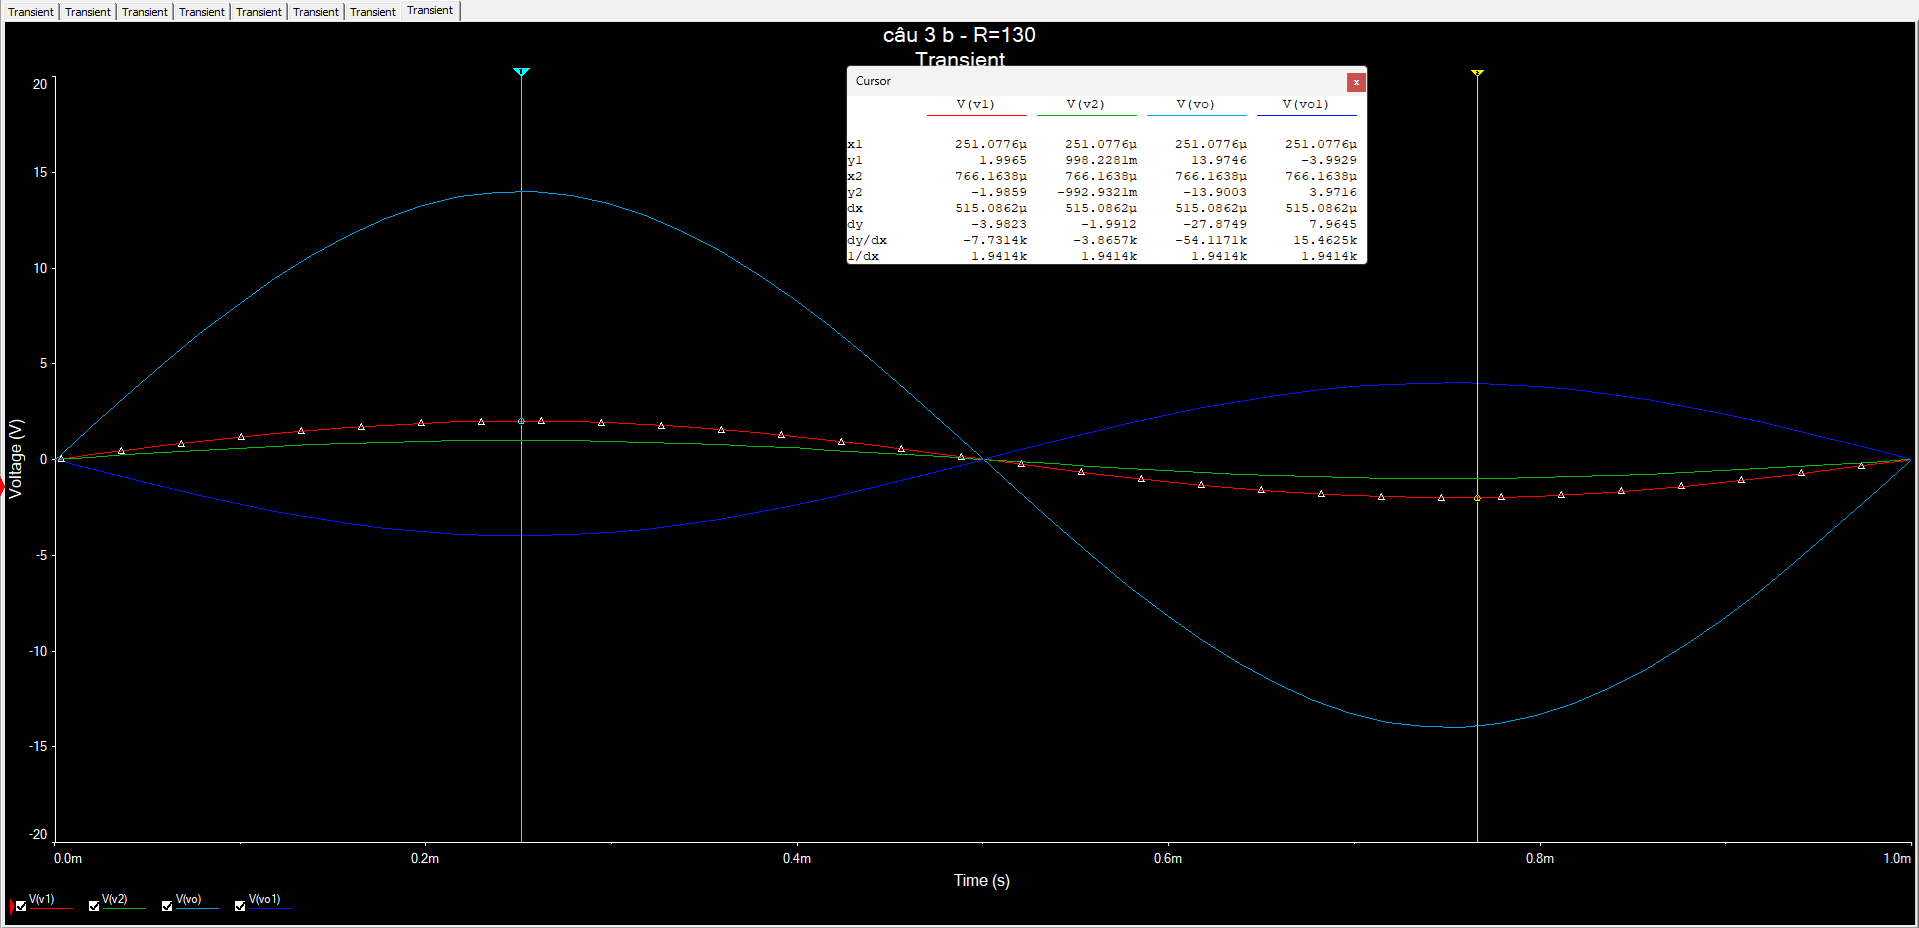
\includegraphics[width=.9\linewidth]{./my-chapters/my-images/Question3/b_songmophong2_nonideal.png}
		\caption{Kết quả mô phỏng liên hệ giữa $V_{o}$ với $V_{1}$ và $V_{2}$ với OPAMP không lý tưởng với việc giảm ảnh hưởng của $I_{ib}$.}
	\end{figure}
	
	\begin{minipage}{.7\linewidth}
		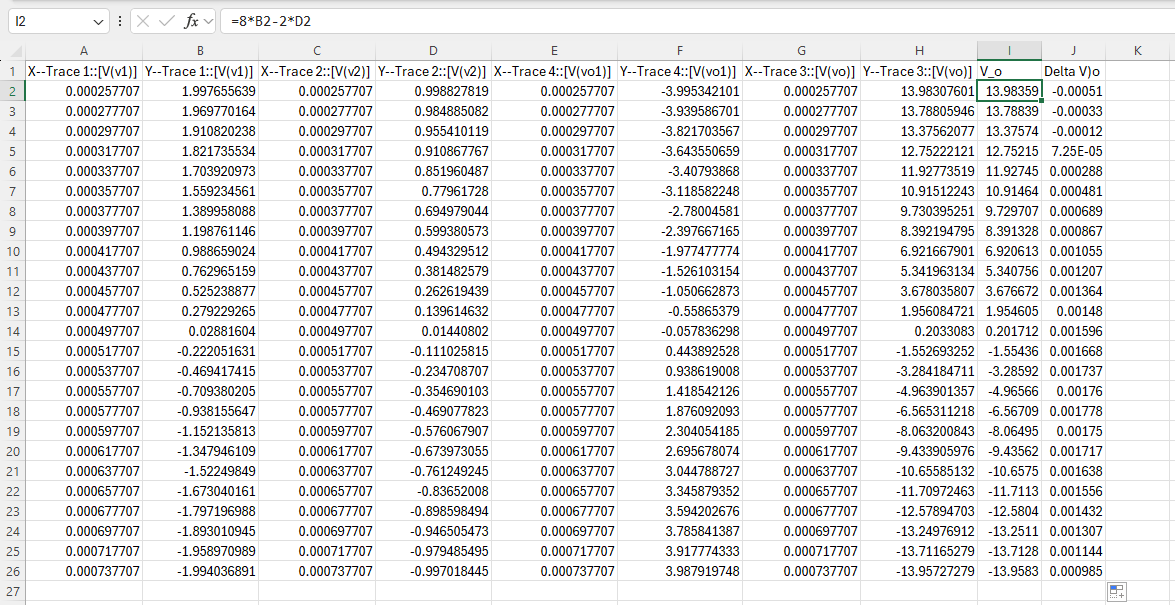
\includegraphics[width=\linewidth]{./my-chapters/my-images/Question3/b_saiso_nonideal_2.png}
	\end{minipage}
	\begin{minipage}{.3\linewidth}
		\begin{itemize}[label=-]
			\item \finalresult{\Delta V_{o_{max}} = 0.001778309 \,\textsf{V}}
			\item \finalresult{\Delta V_{o_{min}} = -0.000513461 \,\textsf{V}}
		\end{itemize}
	\end{minipage}
	
	$\Delta V_{o_{max}}$ và $\Delta V_{o_{min}}$ giảm đáng kể do không có sự can thiệp của $I_{io}$ và $I_{ib}$ vào.
\end{itemize}
